% ******************************* Thesis Annex 1 ********************************

\chapter{Manual de construcción de RAU-Switch}

% **************************** Define Graphics Path **************************
\ifpdf
    \graphicspath{{Anexo1/Figs/Raster/}{Anexo1/Figs/PDF/}{Anexo1/Figs/}}
\else
    \graphicspath{{Anexo1/Figs/Vector/}{Anexo1/Figs/}}
\fi


% *************************** Resumen ***************************************

\section{Resumen}

En este documento se ofrece una guía paso a paso para construir partiendo de una PC de escritorio, una tarjeta NetFPGA-10G y diferentes herramientas de software un switch OpenFlow 1.3 IP/MPLS híbrido; lo que denominamos RAUSwitch.\\

En la misma no se asume ningún conocimiento previo acerca de la plataforma NetFPGA, Xilinx ISE y sobre el protocolo OpenFlow.\\

Cabe destacar que existen diferentes tutoriales y guías para algunas de las diferentes etapas de la construcción del switch. No obstante se pensó este documento como un resumen práctico de todos ellos, de forma de agilizar el proceso de construcción de tal dispositivo para una persona que recien se encuentra familiarizándose con los conceptos aquí tratados.\\

En caso de querer profundizar en alguna de las etapas, se puede recurrir al material (en caso de existir) utilizado para la construcci\'on de esta gu\'ia, siguiendo las referencias indicadas a lo largo de este documento.

% ************************** Antes de empezar ******************************

\section{Plataforma utilizada}
\label{annexI.1}
A continuación se especifican las caracter\'isticas del hardware utilizado en la construcci\'on de RAU-Switch, as\'i como la especificaci\'on de las herramientas de software con sus correspondientes versiones de producto.
 
Se sugiere respetar en la medida que sea posible los mismos conforme a evitar comportamientos inesperados o no contenidos en el alcance de esta guía.\\

\begin{table}[h]\centering
\begin{tabularx}{\textwidth}{|>{\setlength\hsize{1.0\hsize}\setlength\linewidth{\hsize}}X|}
\hline
\multicolumn{1}{|c|}{Hardware}\\
\hline
\begin{itemize}
\item Procesador: Intel Core i7 4770K 3.50GHz
\item Motherboard Asus ROG Maximus VI Formula
\item Fuente Thermaltake TR2 600W ATX 12V 2.3
\item Memoria RAM Kingstom 8GB DIMM DDR3 1333 MHz (x2)
\item Disco duro Seagate 1TB
\end{itemize}\\

\begin{itemize}
\item NetFPGA-10G: 10-Gigabit SFP+ (x4), x8 gen1 PCIe, Xilinx’s Virtex-5 TX240TFPGA
\item Transiever Finisar FTLX8571D3BCL 850nm 13-50
	  Class 1 21CFR1040.10 LN\#50 7\/01
\item Patchcord multimodo OM3 50/125 duplex lc lc 10 metros pvc 2mm
	  il $\leq$ 0.25dB RL $\geq$ 28dB
\item TP-Link Gigabit PCI Express TG-3468\footnote{En el desarrollo del proyecto, para la construcci\'on del laboratorio de pruebas, una tarjeta de red Ethernet en el diseño RAU-Switchpara. Esto se debe a la necesidad de conectarse al equipo mediante un cable Ethernet RJ45, puesto que no se contaba con otros equipos con tarjetas de red \'opticas para realizar las pruebas. Esto quiere decir entonces que esta componente es opcional.}
\end{itemize}\\
\hline
\end{tabularx}
\caption{RAU-Switch, especificaciones de hardware}
\label{table:RAUHSpecs}
\end{table}


\begin{table}[Htl]\centering
\begin{tabularx}{\textwidth}{|>{\setlength\hsize{1.0\hsize}\setlength\linewidth{\hsize}}X|}
\hline
\multicolumn{1}{|c|}{Software}\\
\hline
\begin{itemize}
\item Sistema Operativo: Ubuntu 12.04 LTS release 12.04 precise 3.11.0-15 generic x86\_64
\item Open vSwitch v2.3.9
\item Repositorio NetFPGA v5.0.5
\item Xilinx ISE\_DS\_LIn 13.04\_087xd.3.0
\item SNMP 5.4.3
\item Quagga 0.99.22
\end{itemize}\\
\hline
\end{tabularx}
\caption{RAU-Switch, especificaciones de software}
\label{table:RAUSSpecs}
\end{table}


\newpage
\section{Instalación y configuración}
En esta sección se explica el proceso de instalación y configuración del software necesario para la construcción de RAUSwitch.\\

En cuanto al orden de procedencia esta guía está organizada de la siguiente forma:

\begin{enumerate}
\item Instalación del sistema operativo
\item Instalación de librerías y dependencias
\item Instalación de suite de desarrollo Xilinx ISE SDK
\item Configuración del entorno de desarrollo NetFPGA
\item Pruebas de aceptación del hardware NetFPGA
\item Programación del hardware
\item Instalación de Open vSwitch
\item Instalaci\'on de Quagga
\item Instalaci\'on de agente SNMP
\end{enumerate}

\subsection{Instalación de un sistema operativo}
Para la instalaci\'on del sistema operativo, utilizamos un dvd de instalaci\'on de Ubuntu 12.04 LTS descargado desde la pagina oficial. Para descargar una imagen con el instalador de este sistema se puede recurrir a:

\begin{center}
http://releases.ubuntu.com/12.04/
\end{center}  

En caso de no estar familiarizado con el proceso de instalacion de un sistema operativo recomendamos el siguiente tutorial:

\begin{center}
http://www.ubuntu.com/download/desktop/install-ubuntu-desktop
\end{center}

\subsection{Instalación de librerías y dependencias}
Las siguientes librerías son necesarias por las diferentes herramientas de software utilizadas en el switch: gitk, git-gui, libusb, build-essential, libc6-dev, fxload, autotools-dev, autoconf, uml-utilities, libtool.\\

Para instalarlas abrir una consola y ejecutar los siguientes comandos:\\

\begin{bash}
# sudo apt-get update
# sudo apt-get install gitk git-gui libusb-dev build-essential 
# sudo apt-get install libc6-dev-i386 fxload autotools-dev
# sudo apt-get install autoconf uml-utilities libtool
\end{bash}

En caso de tener en algún momento errores con el comando gmake(por ejemplo “gmake comand not found”), crear un link simbólico entre \textit{gmake} y \textit{make}. Para ello ejecutar en una consola:\\

\begin{bash}
# sudo ln -s /usr/bin/make /usr/bin/gmake
\end{bash}

\subsection{Instalación de suite de desarrollo Xilinx ISE SDK}

La instalación de la suite Xilinx ISE SDK la realizaremos desde el código fuente por lo que primero que nada debemos descargar dichos archivos desde la página oficial de Xilinx. En este trabajo se descargo el siguiente archivo:

\begin{center}
Xilinx\_ISE\_DS\_Lin\_13.4\_087xd.3.0.tar
\end{center}

Luego debemos ir al directorio en donde se tienen descargado dichos archivos y ejecutamos los siguientes comandos:

\begin{bash}
# tar -xvf Xilinx_ISE_DS_Lin_13.4_087xd.3.0.tar
# sudo chmod +x xsetup
# sudo ./xsetup
\end{bash}

De esta forma se ejecuta el asistente de instalación de la suite de Xillinx.\\

Dejamos todas las opciones que marca por defecto con la excepción de la instalación de los drivers para el cable de programación. En este caso destildar el checkbox correspondiente para evitar que la instalación se finalice con errores.\\

Una vez finalizada la instalación de la suite de Xilinx, debemos instalar los drivers para el cable de programación JTag. En particular trabajaremos con un driver proporcionado por terceras partes disponible en un repositorio github.\\

Por defecto la instalación de Xilinx se realizó en el directorio /opt/Xilinx, en caso contrario trabajar en lo que prosigue en el directorio correspondiente.\\

Abrimos una consola y ejecutamos los siguiente:\footnote{Para la arquitectura de la máquina se debe compilar la versión de 64 bits del driver; lo cual se hace por defecto. En caso de trabajar con una arquitectura de 32bits se puede ejecutar el make para 32bits.}\\

\begin{bash}
# cd /opt/Xilinx/
# git clone git://git.zerfleddert.de/usb-driver
# cd usb-driver/
# make
# chmod +x setup_pcusb
# ./setup_pcusb /opt/Xilinx/13.4/ISE_DS/ISE
\end{bash}

Finalmente reiniciamos la PC.

\subsubsection{Configuración de variables de entorno}
Para utilizar la suite de Xilinx es necesario agregar ciertas variables de entorno al sistema. Para ello una alternativa es editar el archivo \textbf{.bashrc} en la consola del usuario root, agregando las siguientes líneas:\\

\begin{bash}
# sudo su
# nano /root/.bashrc

PATH=\$PATH:/opt/Xilinx/13.4/ISE_DS/EDK/bin/lin64
:/opt/Xilinx/13.4/ISE_DS/common/lib/lin64
:/opt/Xilinx/13.4/ISE_DS/ISE/bin/lin64/
:/opt/Xilinx/13.4/ISE_DS/common/bin/lin64
:/opt/Xilinx/13.4/ISE_DS/EDK/gnu/microblaze/lin64/bin

XILINX=/opt/Xilinx/13.4/ISE_DS/ISE/
XILINX_EDK=/opt/Xilinx/13.4/ISE_DS/EDK
XILINXD_LICENSE_FILE=/opt/Xilinx
LD_LIBRARY_PATH=/opt/Xilinx/13.4/ISE_DS/ISE/lib/lin64/
:/opt/Xilinx/13.4/ISE_DS/EDK/lib/lin64

export PATH
export XILINX
export XILINX_EDK
export XILINXD_LICENSE_FILE
export LD_LIBRARY_PATH
\end{bash}

De esta forma queda instalada la suite de Xilinx y los drivers del cable JTag para la programación de las tarjetas.

\subsubsection{Ejecución de herramientas de la suite de Xilinx}
Para la ejecución de cualquier herramienta de la suite Xilinx es necesario ejecutar un script de configuración, presente en el directorio de instalación de la herramienta. Para ello abrir una consola y ejecutar lo siguiente:\\

\begin{bash}
# /opt/Xilinx/13.4/ISE_DS/settings64.sh
\end{bash}

En caso de que el archivo \textbf{setting64.sh} no cuente con permisos de ejecución asignárselos.\\ 

Luego se puede ejecutar cualquier herramienta de la suite Xilinx, como por ejemplo la herramienta Impact para programar normalmente las tarjetas de la siguiente forma:\\

\begin{bash}
# impact
\end{bash}

\subsubsection{Instalación de licencias de usuario}
Para trabajar con las herramientas de Xilinx es necesario contar con licencias correspondientes para cada una de ellas y en particular dependiendo del tipo de hardware con el que se trabaje dependerá el tipo de licencia necesaria. En nuestro caso se necesita una licencia completa(full license), y vale la pena destacar que con una licencia de prueba no se cuentan con las licencias apropiadas para compilar los proyectos de NetFPGA con los que se trabajar\'a.\\

Para obtener una licencia full se debe ir al sitio de Xilinx de gestión de licencias, registrarse y comprar una licencia full.\\

Asumiendo que ya se tiene descargada una licencia full, para cargar la misma abrir una consola y ejecutar lo siguiente:\\

\begin{bash}
# /opt/Xilinx/13.4/ISE_DS/common/bin/lin64/xlcm
\end{bash}

Una vez que se ejecuta el comando anterior, se abrirá el programa  Xilinx Lincense Configuration Manager, que es el asistente de licencias de la suite de Xilinx. Una vez abierto el mismo ir a la pestaña de Manejo de Licencias (Manage Xilinx Licenses) e importar los archivos de licencias \emph{.lic} obtenidos(botón copy license).

Una vez importada la licencia se podrán ver abajo las diferentes características que proveen las licencias cargadas. En caso de que no se actualice la pestañea apretar el botón \textbf{Refresh}.


\subsection{Configuración del entorno de desarrollo NetFPGA}
A continuación se explica como acceder al código fuente de NetFPGA y como empezar a programar el hardware con el mismo.\\

Naturalmente lo primero que debemos hacer es obtener el código fuente con las implementaciones de proyectos y herramientas, para lo cual es necesario crearse un usuario github y luego registrarse como desarrollador NetFPGA en el sitio oficial. Este último proceso puede llevar algunas horas dado que el proceso de aceptación se realiza manualmente.\\

Para registrarse como desarrollador NetFPGA completar el siguiente formulario:

\begin{center}
http://netfpga.org/2014/\#/10G\_going\_beta/
\end{center}

Una vez aceptada la solicitud de unirse al equipo de NetFPGA, se tendrá acceso a los repositorios de código fuente en github. Descargamos la versión base de código fuente en el sitio de NetFPGA en github.

Para descargar el código fuente basta con acceder al siguiente link estando logueado en Github:

\begin{center}
https://github.com/NetFPGA/NetFPGA-10G-live/tags
\end{center}

En particular trabajaremos con la release 5.0.5 la cual se encuentra accesible mediante el siguiente enlace:
 
\begin{center}
https://github.com/NetFPGA/NetFPGA-10G-live/releases/tag/release\_5.0.5
\end{center}

Una vez descargado el código fuente descomprimimos el archivo .zip en un directorio a elección(en nuestro caso utilizaremos el directorio /home/mina). Luego abrimos una consola en el directorio y ejecutamos lo siguiente:

\begin{bash}
# cd /home/mina/NetFPGA-10G-live-release\_5.0.5/
# make cores
\end{bash}

Este proceso puede llevar de 5 a 10 minutos dependiendo de las prestaciones del hardware. Una vez finalizado el proceso anterior estamos en condiciones de programar las tarjetas NetFPGA con el proyecto que creamos conveniente.

\subsection{Pruebas de aceptación del hardware NetFPGA}
Antes de empezar a trabajar con el hardware NetFPGA y en especial a programarlo con cualquier proyecto, es sumamente importante ejecutar un conjunto de pruebas desarrolladas específicamente para la tarjeta NetFPGA-10G, con el objetivo de chequear el correcto funcionamiento de sus componentes. En particular existen dos pruebas:

\begin{itemize}
\item RLDRAM Test\citep{NetFPGA5}
\item Production Test\citep{NetFPGA7}
\end{itemize}

Estos tests son proyectos de referencia; es decir fueron desarrollados por NetFPGA y la universidad de Stanford. Con los mismos se programan las tarjetas, de igual forma que se programaría cualquier otro proyecto, y luego se ejecutan una serie de scripts que realizan pruebas y verificaciones en el hardware. En pocas palabras, además de verificar el correcto funcionamiento de las tarjetas, al ejecutar los test se tiene una primera experiencia programando el hardware.\\

Es importante tener en cuenta que las tarjetas NetFPGA pueden funcionar tanto conectadas a una PC (escenario elegido) denominado server mode como conectadas solamente a una fuente de poder denominado standalone mode.\\

En particular, ambos proyectos de pruebas pueden programarse para ejecutarse en ambas modalidades de funcionamiento. En esta guía se explica como programar y ejecutar dichos proyectos bajo el modo de funcionamiento servidor. En caso de requerirse de una ejecuci\'on de pruebas en modo standalone puede encontrarse en\citep{NetFPGA6}\citep{NetFPGA8} una guía detallada.

\subsubsection{Programación y ejecución del Production Test}
A continuación se detalla el procedimiento para programar el hardware con el test de producción y luego ejecutar el conjunto de pruebas asociadas. Esta guía esta basada a su vez en una guía mas completa accesible en\citep{NetFPGA6}\\

EL primer paso para programar el test de producción es configurar la tarjeta NetFPGA-10G correctamente, así como instalarla en una PC. Es sumamente IMPORTANTE seguir cuidadosamente cada una de las indicaciones que aquí se mencionan para lograr los resultados correctos y no dañar el hardware en el proceso de manipulación.\\ 

La tarjeta necesita un suministro de corriente mediante el conector ATX para poder funcionar. A continuación se describe como instalar el hardware:

\begin{itemize}
\item Asegurarse que el jumper J16 no esta activado. Este Jumper se encuentra en la esquina superior izquierda de la tarjeta, en la cercanía del conector RS232 DB-9(figura~\ref{fig:Img1}.

\begin{figure}[htbp!] 
\centering    
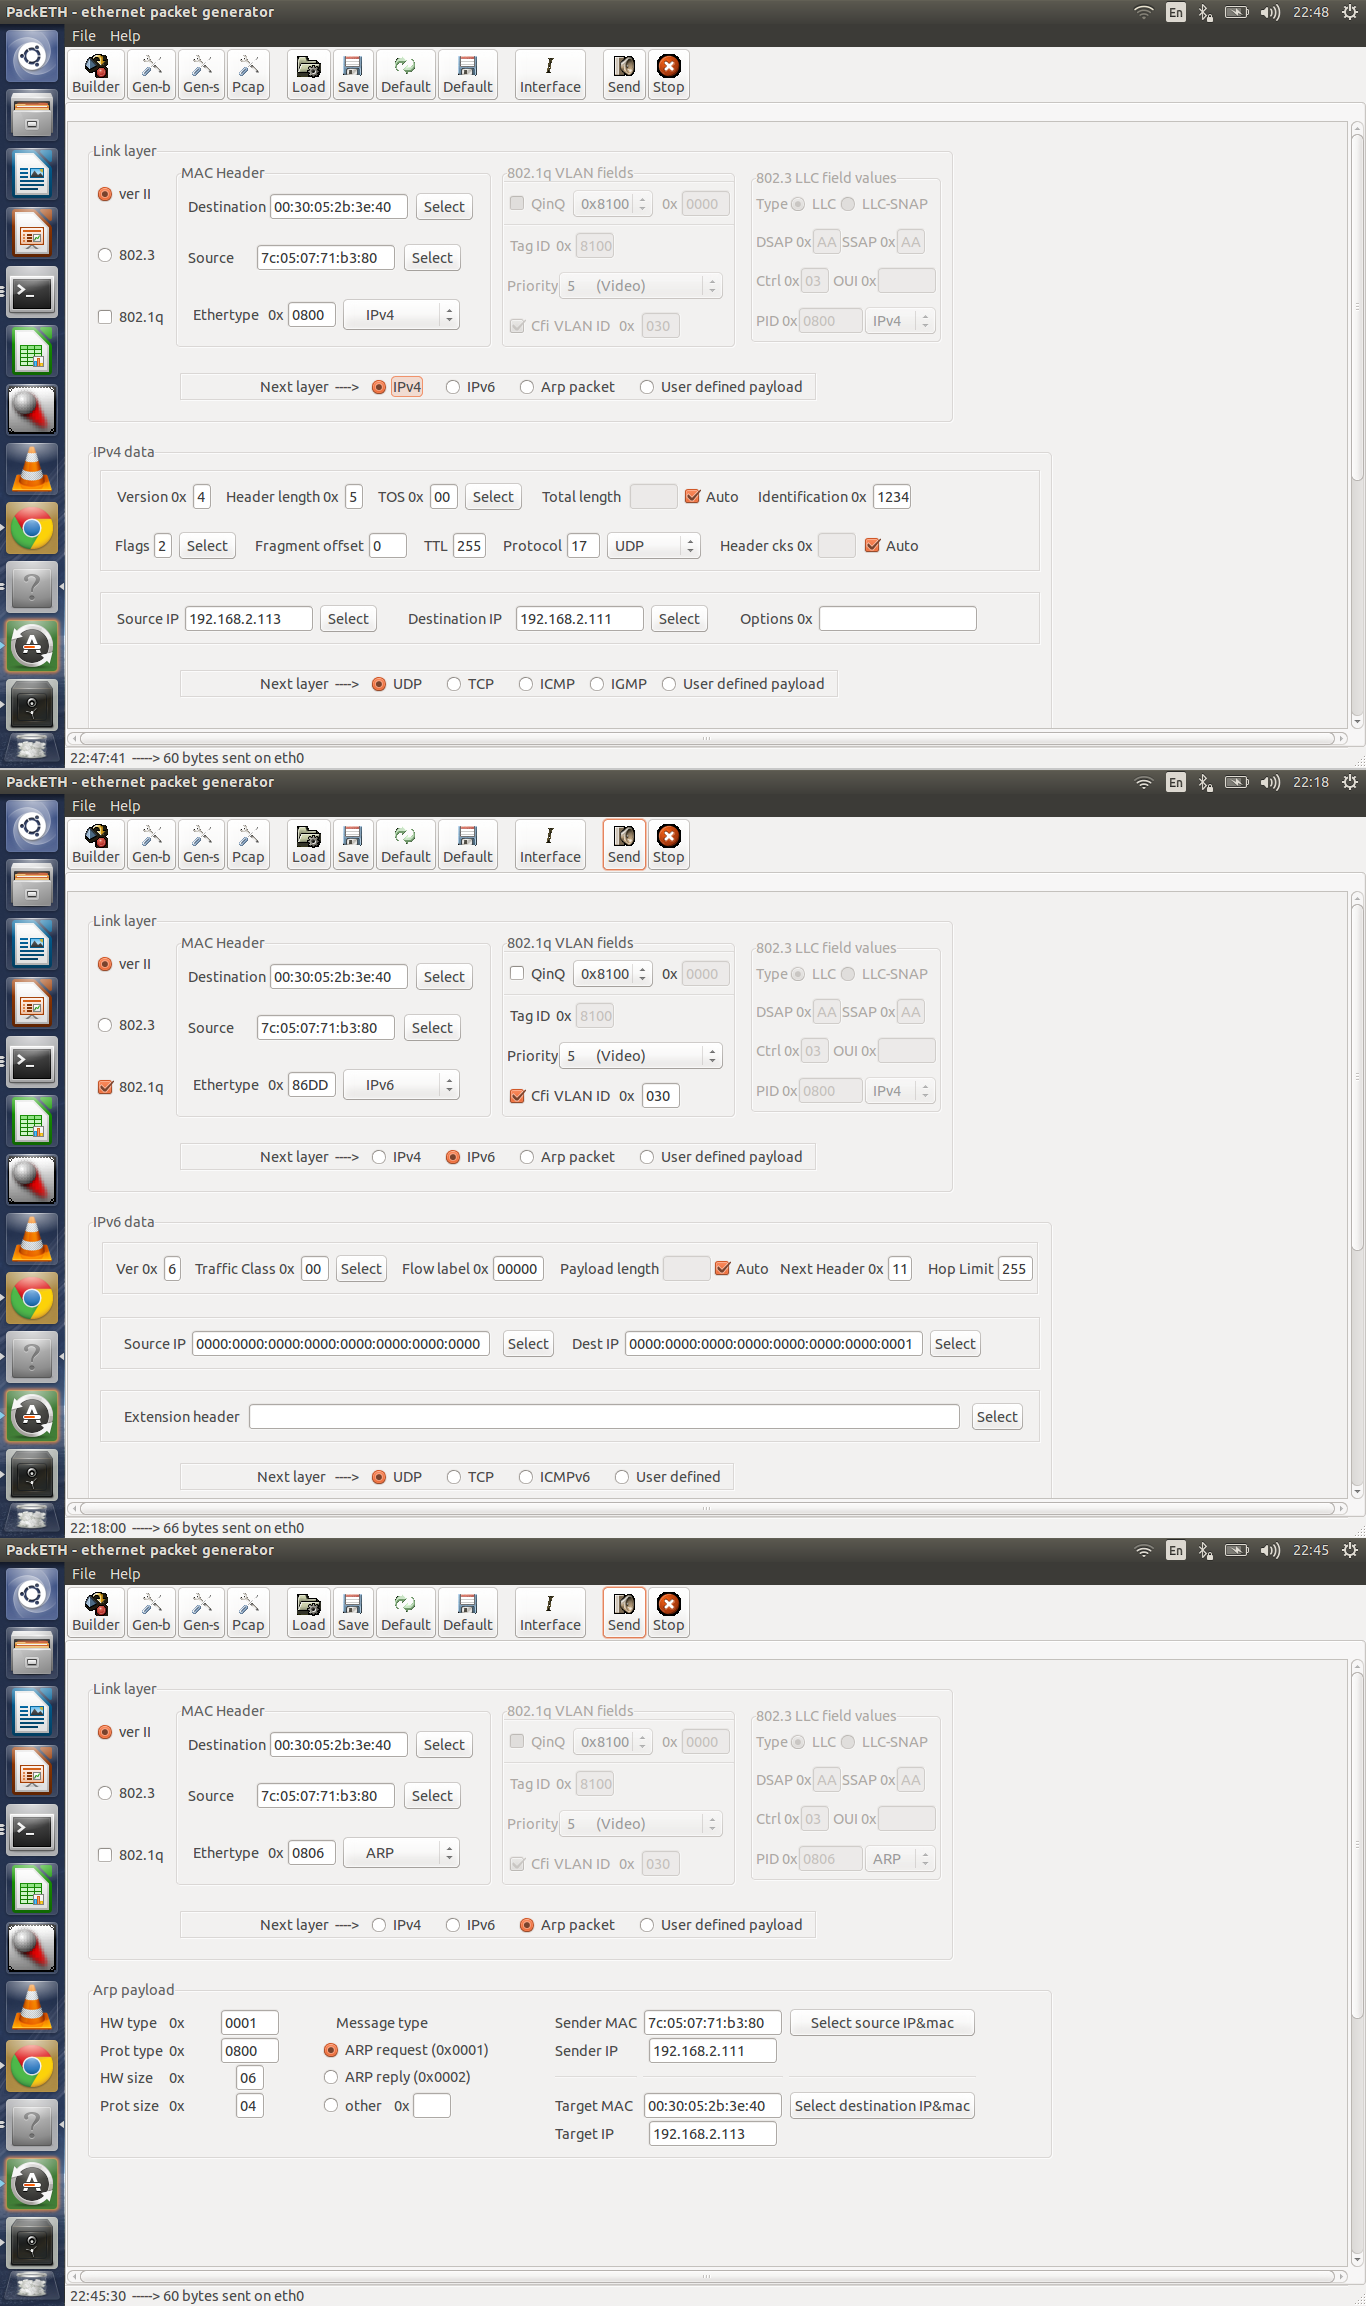
\includegraphics[width=0.50\textwidth]{Img1}
\caption[Jumper J16]{Jumper J16, Imagen extra\'ida de \citep{NetFPGA6}}
\label{fig:Img1}
\end{figure}

\item Setear el switch SW9 en la posición PCIe. Asegurarse bien de que el switch esta completamente puesto en dicha posición(figura ~\ref{fig:Img2}).

\begin{figure}[htbp!] 
\centering    
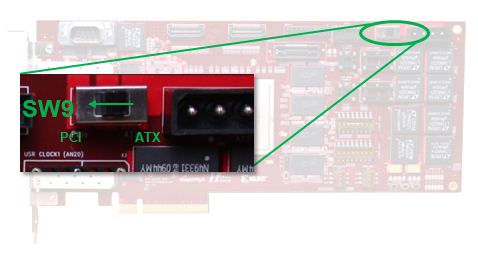
\includegraphics[width=0.50\textwidth]{Img2}
\caption[SW9 en posicion PCIe]{SW9 en posicion PCIe, Imagen extra\'ida de \citep{NetFPGA6}}
\label{fig:Img2}
\end{figure}

\item Asegurarse que los switches DIP SW1, SW2, SW6 y SW10 están correctamente seteados acorde al siguiente esquema(figura ~\ref{fig:Img3}):\\

\textbf{SW1:} SEL0, SEL1, M2, M1, M0, N2, N1, N0 son seteados en off, off, off, on, on, on, off, off\\
\textbf{SW6:} SEL0, SEL1, M2, M1, M0, N2, N1, N0 son seteados en off, off, off, on, off on, off, on\\
\textbf{SW3:} M0, M1, M2 son seteados en on, on, on\\
\textbf{SW10:} SEL0, SEL1, SEL2 son seteados en on, off, off\\

\begin{figure}[htbp!] 
\centering    
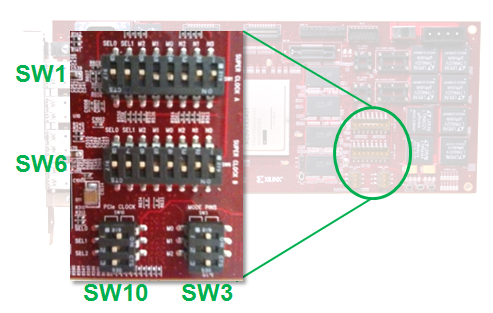
\includegraphics[width=0.50\textwidth]{Img3}
\caption[Posiciones DIP SW1 SW2 SW6 SW10]{Posiciones DIP SW1 SW2 SW6 SW10, Imagen extra\'ida de \citep{NetFPGA6}}
\label{fig:Img3}
\end{figure}

\item Con la PC apagada y desconectada de la electricidad instalar la tarjeta NetFPGA-10G en un slot PCIe disponible.

\item Conectar alguno de los conectores ATX disponibles de la PC al conector ATX de la tarjeta NetFPGA-10G(figura ~\ref{fig:Img4}).

\begin{figure}[htbp!] 
\centering    
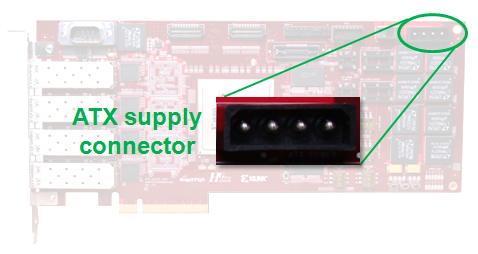
\includegraphics[width=0.50\textwidth]{Img4}
\caption[Conector ATX]{Conector ATX, , Imagen extra\'ida de \citep{NetFPGA6}}
\label{fig:Img4}
\end{figure}

\item Conectar el cable Samtec Twinax a la interfaz de expansión de la tarjeta formando un “loop”( figura ~\ref{fig:Img5})

\newpage
\begin{figure}[htbp!] 
\centering    
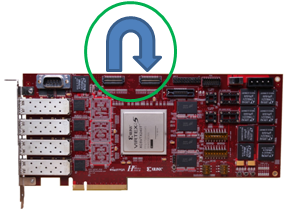
\includegraphics[width=0.40\textwidth]{Img5}
\caption[Cable samtec twinax]{Cable samtec twinax, , Imagen extra\'ida de \citep{NetFPGA6}}
\label{fig:Img5}
\end{figure}

\item Conectar un par de cables 10GE SFP+ a las interfaces de la tarjeta. Cada cable conecta dos puertos adyacentes formando dos “bucles”(ver figura ~\ref{fig:Img6}):

\begin{figure}[htbp!] 
\centering    
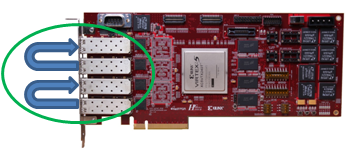
\includegraphics[width=0.50\textwidth]{Img6}
\caption[Cables samtec twinax conectados]{Cables samtec twinax conectados}
\label{fig:Img6}
\end{figure}

\item Conectar un cable serial RS232 al puerto serial RS232 en la tarjeta. Conectar el otro extremo en el puerto serial COM de la PC o a un adaptador USB por ejemplo(ver figura ~\ref{fig:Img7}).

\begin{figure}[htbp!] 
\centering    
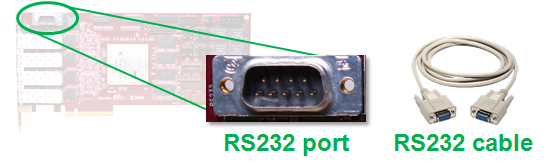
\includegraphics[width=0.50\textwidth]{Img7}
\caption[Cable serial puerto COM]{Cable seria puerto COM, Imagen extra\'ida de \citep{NetFPGA6}}
\label{fig:Img7}
\end{figure}

\item Conectar el cable de programación Xilinx JTAG al conector JTAG en la tarjeta. Luego conectar el otro extremo a la PC a través de un puerto USB por ejemplo(figura ~\ref{fig:Img8}).

\newpage
\begin{figure}[htbp!] 
\centering    
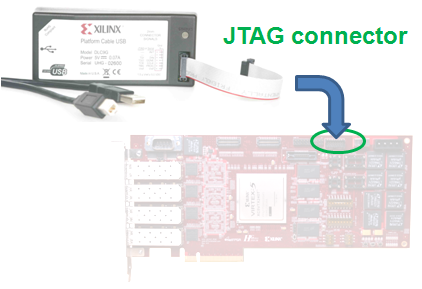
\includegraphics[width=0.55\textwidth]{Img8}
\caption[Cable JTAG]{Cable JTAG, Imagen extra\'ida de \citep{NetFPGA6}}
\label{fig:Img8}
\end{figure}

\end{itemize}

Al finalizar, la tarjeta NetFPGA debería estar instalada como se muestra en la siguientes figuras~\ref{fig:Img9}~\ref{fig:Img10}:

\begin{figure}[htbp!] 
\centering    
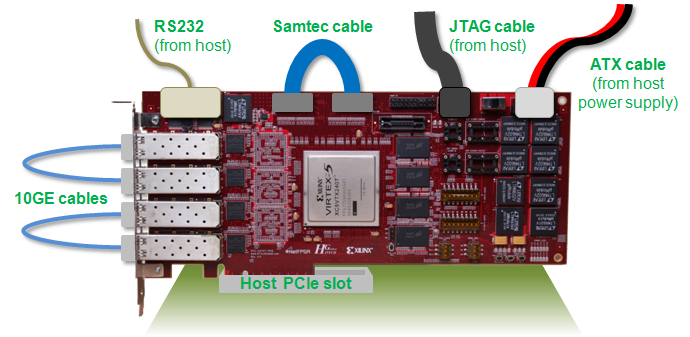
\includegraphics[width=0.80\textwidth]{Img9}
\caption[Tarjeta NetFPGA esquema de instalación]{Tarjeta NetFPGA esquema de instalación, Imagen extra\'ida de \citep{NetFPGA6}}
\label{fig:Img9}
\end{figure}

\newpage
\begin{figure}[htbp!] 
\centering    
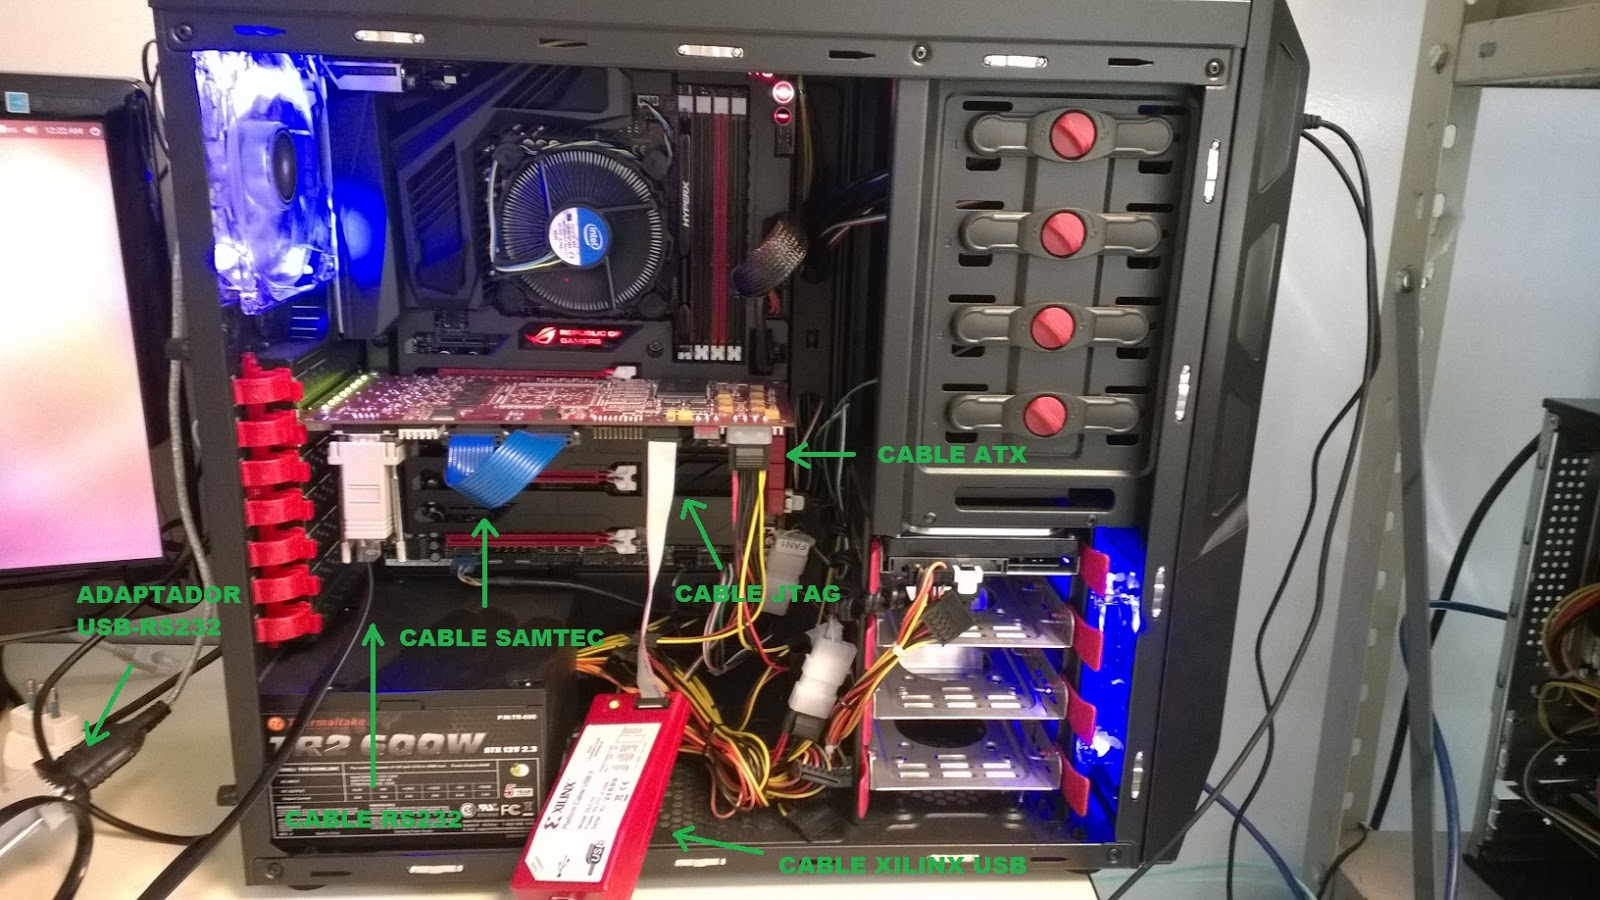
\includegraphics[width=0.85\textwidth]{Img10}
\caption[Tarjeta NetFPGA instalada en una PC]{Tarjeta NetFPGA instalada en una PC}
\label{fig:Img10}
\end{figure}

Para ejecutar el Test de Producción seguir los siguientes pasos:

\begin{itemize}
\item Encender el PC y como usuario root abrir el archivo /boot/grub/grub.cfg con un editor de texto. Realizar las siguientes modificaciones:

\begin{itemize}
\item Localizar la entrada particular para la distribución del kernel que se tenga
\item Encontrar la línea que comienza con Kernel
\item Concatenar \textbf{memmap=256M\$0x5f700000} al final de la línea(ver figura ~\ref{fig:Img11}).\\
El parámetro memmap=256M\$0x5f700000 es pasado al kernel al momento de iniciar el sistema. El mismo reserva una región de 256MB de memoria disponible comenzando en la dirección 0x5f700000. Este bloque es utilizado posteriormente en el Test PCIe DMA.
\item Guardar los cambios realizados al archivo

\newpage
\begin{figure}[htbp!] 
\centering    
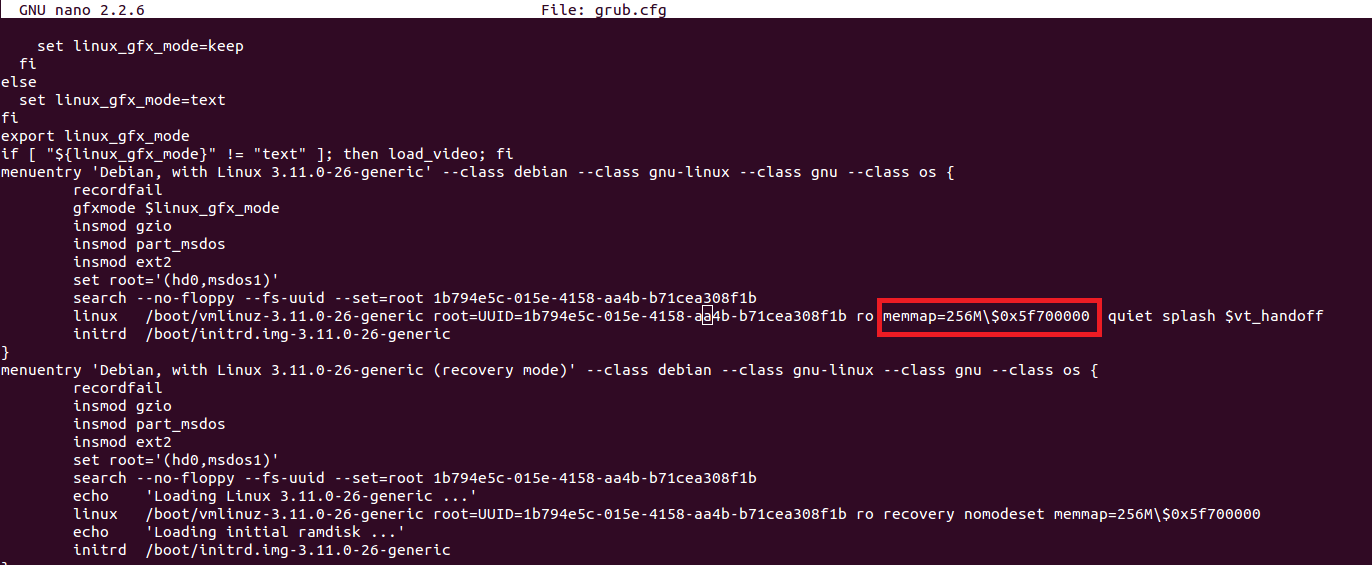
\includegraphics[width=0.95\textwidth]{Img11}
\caption[Reserva de bloque de memoria]{Reserva de bloque de memoria}
\label{fig:Img11}
\end{figure}

\end{itemize}

\item Iniciar la aplicación IMPACT de Xilinx indicando la opción “Yes” cuando se pregunte si queremos que la herramienta cree y guarde automáticamente un proyecto por nosotros.

\item Programar la CPLD con el diseño localizado en el directorio(ver figura ~\ref{fig:Img12})\\ 
/NF\_ROOT/projects/production\_test/bitfiles/cpld.jed

\begin{figure}[htbp!] 
\centering    
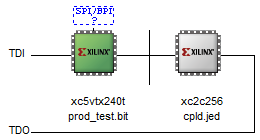
\includegraphics[width=0.45\textwidth]{Img12}
\caption[Programación Impact]{Programación Impact}
\label{fig:Img12}
\end{figure}

\item Programar la FPGA con el bitstream localizado en el directorio\\
/NF\_ROOT/projects/production\_test/bitfiles/prod\_test\_no\_rldram.bit

IMPACT posiblemente nos pregunte si queremos asociar un dispositivo PROM, seleccionar qué no. Programar la tarjeta puede llevar algún tiempo; de 10 a 20 minutos dependiendo del proyecto. Este proyecto en particular no debería tomar más de 10 minutos.

\item Reiniciar la PC

\item Verificar que el bloque de memoria DMA ha sido reservado correctamente a través de los siguientes pasos:

\begin{itemize}
\item Ejecutar en una consola:
\begin{bash}    
# cat /proc/cmdline
\end{bash}    
  
\item La salida debería ser similar a la figura ~\ref{fig:Img13}

\begin{figure}[htbp!] 
\centering    
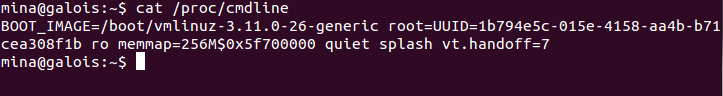
\includegraphics[width=0.85\textwidth]{Img13}
\caption[Reserva bloque de memoria]{Reserva bloque de memoria}
\label{fig:Img13}
\end{figure}

\end{itemize}

\item Verificar que la tarjeta ha sido correctamente instalada siguiendo los siguientes pasos:

\begin{itemize}
\item Desde una consola verificar el dispositivo NetFPGA-10G ejecutando:
\begin{bash}
#lspci | grep Xilinx
\end{bash}

\item La salida debería ser similar a:
\begin{bash}
# 01:00.0 Ethernet controller: Xilinx Corporation Device 4244
\end{bash}

\end{itemize}

\item Desde la PC ejecutar el test de producción a través de los siguientes pasos:

\begin{itemize}
\item Situarse en la carpeta del Test de Producción
\begin{bash}
# cd projects/production_test/sw/
\end{bash}

\item Compilar el test
\begin{bash}
# make
\end{bash}

\item Posicionarse en la carpeta de scripts
\begin{bash}
# cd scripts
\end{bash}

\item Ejecutar el Test de Producción
\begin{bash}
# sudo ./production_test.py
\end{bash}

La salida debería ser como la que se muestra a continuación(ver figura ~\ref{fig:Img14}):

\newpage
\begin{figure}[htbp!] 
\centering    
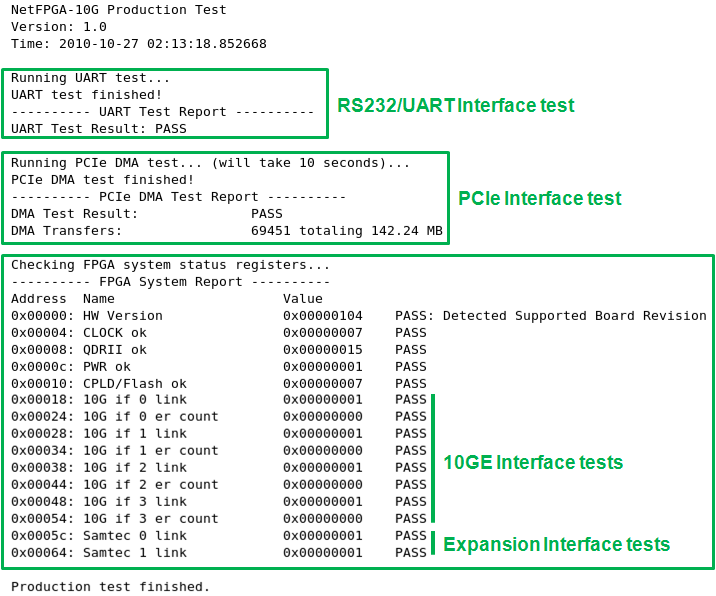
\includegraphics[width=0.95\textwidth]{Img14}
\caption[Test de Producción salida esperada]{Test de Producción salida esperada}
\label{fig:Img14}
\end{figure}
\end{itemize}

\end{itemize}

Para ejecutar el RLDRAM Test recomendamos utilizar la guía \citep{NetFPGA8}.

\subsection{Programación de la tarjeta}

A continuación se describen los pasos necesarios para programar las tarjetas NetFPGA en particular con el proyecto ReferenceNIC. En lo que prosigue se utiliza NF\_ROOT para referirse al directorio donde se encuentra descargado el código fuente de NetFPGA.

\subsubsection{Configuración de la tarjeta}
Antes de comenzar, es necesario realizar algunas modificaciones en el hardware NetFPGA para habilitar la programación pcie del mismo, utilizada en la programación persistente.\\ 

Para habilitar la programación PCI, es necesario cambiar la posición del switch Disp SW3 desde la posición por defecto (M0:On, M1:On, M2:On) a la posición de programación PCIE(M0:Off, M1:On, M2:On). Esta configuración habilita tanto la programación de la tarjeta por el cable de programación JTAG como por la interfaz PCIe.\\

La siguiente figura muestra la posición del Dip SW3 en la configuración PCIe(ver figura ~\ref{fig:Img15}).

\begin{figure}[htbp!] 
\centering    
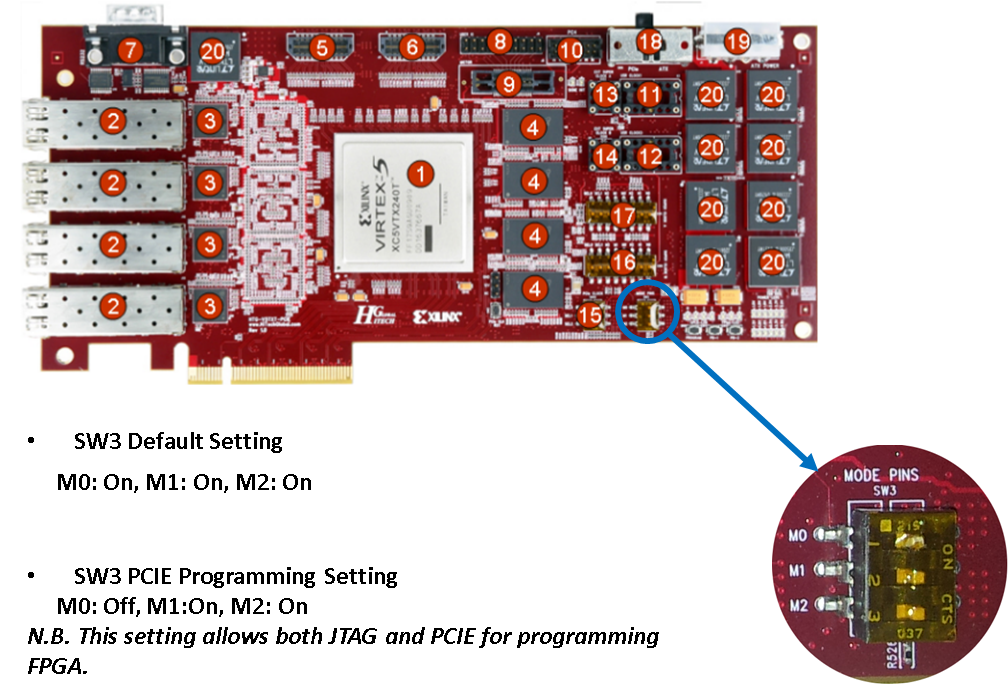
\includegraphics[width=0.95\textwidth]{Img15}
\caption[Configuración SW3 JTag/PCIe programing]{Configuración SW3 JTag/PCIe programing}
\label{fig:Img15}
\end{figure}

Recordar que los cambios a la configuración de la tarjeta se deben realizar con la PC apagada y sin conexión a la corriente eléctrica para evitar daños en el hardware.\\

Una vez configurada la tarjeta conectar la PC a la corriente eléctrica y encender la misma.

\subsubsection{Programación de la tarjeta}
Antes que nada es necesario realizar algunos cambios en archivos del código fuente asociados a los proyectos NetFPGA utilizados, arreglando algunos errores reportados para la version de código fuente utilizada en este manual. Entonces en caso de trabajar con la versión 5.0.5 (recomendada) se deben realizar las siguientes modificaciones:

\begin{enumerate}

\item En el directorio NF\_ROOT/projects/reference\_nic/hw/ cambiar en el archivo \textit{system.mhs} lo siguiente:

\begin{bash}
PORT axi_emc_0_Mem_DQ_pin = axi_emc_0_Mem_DQ, DIR = IO, 
VEC = [*7*:0]
\end{bash}

cambiar por

\begin{bash}
PORT axi_emc_0_Mem_DQ_pin = axi_emc_0_Mem_DQ, DIR = IO, 
VEC = [*31*:0]
\end{bash}

\item En el directorio NF\_ROOT/projects/reference\_nic/hw/nf10 cambiar en el archivo \textit{xflow.opt} lo siguiente: 

\begin{bash}
-t *1*
\end{bash}

cambiar por

\begin{bash}
-t *5*
\end{bash}

(*) Los “*” no van

\item Modificar el driver utilizado por el proyecto ReferenceNIC:
\begin{enumerate}
\item Posicionarse en el directorio NF\_ROOT/projects/reference\_nic/sw/host/driver
\item Abrir el archivo nf10\_phy\_conf.c y comentar las líneas 217,219 y 240
\end{enumerate}

\end{enumerate}

Finalmente se debe compilar el proyecto. Para ello en una consola ejecutamos

\begin{bash}
# cd NetFPGA_ROOT/projects/reference_nic
# make
# cd cpld
# make
\end{bash}

Este proceso puede llevar de 10 a 20 minutos.\\

Ahora programamos la tarjeta NetFPGA con el proyecto ReferenceNIC, para lo cual es necesario conectar el cable de programación JTag a la tarjeta y a la PC.\\

Luego en una consola se ejecuta lo siguiente:

\begin{bash}
# cd NetFPGA_ROOT
# cd tools/scripts
# ./impact_run 
  ../../projects/reference_nic/bit/reference_nic.bit 
  ../../projects/reference_nic/cpld/cpld.jed 
\end{bash}

(*) En caso de que aparezca el error “NF\_ROOT or NF\_DESIGN\_DIR variable is not defined”
abrir el script impact\_run.sh y definir una variable de nombre NF\_ROOT con el valor del directorio donde esta instalado el código fuente de NetFPGA.\\

Luego de finalizada la ejecución del comando reiniciar la máquina. Es sumamente importante que se reinicie y no que se apague, puesto que hasta el momento solo se ha programado el hardware en forma volátil. Esto quiere decir que producirse un corte de corriente el misma se desprogramaría.\\

Una vez reiniciada la PC es necesario cargar el driver del ReferenceNIC en el kernel del sistema. Para ello posiblemente primero se deba compilar el driver. Para compilar el driver ejecutar en una consola:\\

\begin{bash}
# cd NetFPGA_ROOT/projects/reference_nic/sw/host/driver
# make
# insmod nf10.ko
\end{bash}

Ahora vamos a programar una de las memorias flashes de la tarjeta (en particular utilizaremos la unidad A con el proyecto ReferenceNIC, de forma de hacer persistente la programación de la tarjeta.

Para ello en una consola ejecutamos:

\begin{bash}
# cd NF_ROOT/projects/reference_nic/bitfiles
# ./bit2bin.sh reference_nic.bit
\end{bash}

Con lo anterior se genera un archivo binario a partir del bitfile del proyecto, con el que programaremos la memoria. Luego de este comando se deberían de haber creado 3 archivos

\begin{itemize}
\item reference\_nic.prm
\item reference\_nic.bin
\item reference\_nic.cfi
\end{itemize}

Luego ejecutamos lo siguiente:

\begin{bash}
# cd ../sw/host/pcieprog
# ./nf10_configure -b ../../../bitfiles/reference_nic.bin -f a
\end{bash}

Apagamos la PC y la volvemos a prender. Ahora el chip FPGA de la tarjeta se encuentra programado a partir del contenido de la memoria flash A, con el proyecto que allí grabamos.\\

Para no cargar el driver del ReferenceNIC cada vez que se reinicie la máquina podemos modificar el archivo /etc/rc.local agregando la siguiente línea:

\begin{bash}
insmod NF_ROOT/preojects/reference_nic/sw/host/driver/nf10.ko
\end{bash}

\subsection{Instalación de Open vSwitch}
Open vSwitch(ovs) lo instalaremos también desde su código fuente, por ejemplo ejecutando lo siguiente en una consola:

\begin{bash}
# wget http://openvswitch.org/releases/openvswitch-2.3.0.tar.gz
# tar zxvf openvswitch-2.3.0.tar.gz
# cd openvswitch-2.3.0
#./boot.sh
#./configure --with-linux=/lib/modules/\$(uname -r)/build
\end{bash}

Luego se compila el código fuente:

\begin{bash}
# make && make install
\end{bash}

Se inserta en el kernel de linux el módulo de ovs

\begin{bash}
# cd datapath/linux
# modprobe openvswitch
\end{bash}

Podemos verificar que el módulo se insertó correctamente de la siguiente forma:

\begin{bash}
# lsmod | grep openvswitch

openvswitch    57291      0  
gre         14236         1     openvswitch
\end{bash}

Luego creamos el siguiente directorio necesario para la configuración del ovs:

\begin{bash}
# mkdir -p /usr/local/etc/openvswitch
\end{bash}

Finalmente creamos la base de datos de configuración de ovs:

\begin{bash}
# ovsdb-tool create /usr/local/etc/openvswitch/conf.db 
vswitchd/vswitch.ovsschema
\end{bash}

Ya se esta en condiciones de levantar cualquiera de los demonios de ovs. En particular para iniciar ovs debemos indicar una serie de parámetros como la base de datos donde se encuentra la configuración, en caso de utilizar una conexión segura con el controlador los certificados SSL correspondiente entre otras cosas. Para ello es conveniente crear un script como el siguiente:

\begin{bash}
ovsdb-server /usr/local/etc/openvswitch/conf.db \
--remote=punix:/usr/local/var/run/openvswitch/db.sock \
--remote=db:Open_vSwitch,Open_vSwitch,manager_options \
--private-key=db:Open_vSwitch,SSL,private_key \
--certificate=db:Open_vSwitch,SSL,certificate \
--bootstrap-ca-cert=db:Open_vSwitch,SSL,ca_cert 
--pidfile --detach --log-file

ovs-vsctl --no-wait init
ovs-vswitchd --pidfile --detach
ovs-vsctl show

\end{bash}

Por simplicidad hemos comentado las líneas relacionadas a la parte de seguridad en la comunicación entre el ovs y el controlador.\\

Finalmente para automatizar la carga de los drivers de Open vSwitch al encender la PC, crear una carpeta de nombre ovs dentro del directorio /lib/modules/\$(uname -r)/kernel/drivers
como se muestra a continuación.

\begin{bash}
# mkdir /lib/modules/$(uname -r)/kernel/drivers/ovs
# cd /lib/modules/$(uname -r)/kernel/drivers/ovs    
\end{bash}

Posteriormente copiar los archivos de extensión .o y .ko dentro de la carpeta de instalaci\'on de ovs(llamemos le OVS\_ROOT) en el siguiente directorio \\ OVS\_ROOT/datapath/linux al directorio anteriormente creado.\\

Finalmente ejecutamos el siguiente comando para actualizar las listas de dependencias para cada módulo agregado.

\begin{bash}
# depmod
\end{bash}

\subsection{Instalación de software de ruteo Quagga}
El software de ruteo Quagga puede instalarse con un gestor de aplicaciones(apt-get) o desde su codigo fuente; en este tutorial utilizamos esta ultima opción. 

El código fuente podemos obtenerlo desde el sitio oficial de quagga:

\begin{center}
http://www.nongnu.org/quagga/
\end{center}
 
o desde el siguiente link:

\begin{center}
http://www.nongnu.org/quagga/docs/docs-info.html\#OSPFv2
\end{center}

Una vez descargado el código fuente descomprimimos el archivo quagga.public-master.zip en el directorio deseado. En este caso utilizaremos el directorio /home/mina como venimos haciendo para el resto del software instalado. Luego abrimos una consola y ejecutamos los siguientes comandos para compilar el código fuente:

\begin{bash}
# ./configure
# make 
\end{bash}

\subsection{Instalaci\'on de agente SNMP}
Para la instalaci\'on del agente SNMP se utiliza simplemente el gestor de paquetes de Ubuntu \textbf{apt-get}(en otras plataformas se podr\'ia utilizar por ejemplo opkg o yum).

Por lo tanto para instalar el agente SNMP ejecutamos en una consola lo siguiente:

\begin{bash}
# apt-get install snmp snmpd
\end{bash}

\subsection{Extra}

